
\chapter{PENGUJIAN DAN PEMBAHASAN}
Pada bab pengujian dan pembahasan ini, penulis akan melakukan pengujian sistem kendali\textit{ arm manipulator} robot SCARA berdasarkan spesifikasi sistem yang telah dijelaskan pada bab sebelumnya. Tujuan pengujian ini adalah untuk membuktikan apakah sistem yang diimplementasikan telah memenuhi spesifikasi dan rancangan yang sudah direncanakan sebelumnya. Hasil dari pengujian akan dimanfaatkan untuk menyempurnakan kinerja dari sistem dan sekaligus digunakan dalam pengembangan sistem lebih lanjut. Metode pengujian dipilih berdasarkan fungsionalitas dan beberapa parameter yang ingin diketahui dari sistem tersebut. Data yang diperoleh dari metode pengujian yang dipilih tersebut dapat memberikan informasi yang cukup dan dapat digunakan untuk penyempurnaan dan pengembangan sistem.

Metode pengujian menggunakan dua macam metode, yaitu pengujian fungsionalitas dari setiap komponen dan pengujian sistem secara keseluruhan. Pengujian fungsionalitas digunakan untuk membuktikan apakah sistem yang diimplementasikan dapat memenuhi persyaratan dari fungsi operasional yang telah dirancang dan direncanakan sebelumnya. Sedangkan pengujian sistem secara keseluruhan bertujuan untuk memperoleh beberapa parameter yang dapat menunjukkan kemampuan dan keandalan dari sistem secara keseluruhan dalam menjalankan fungsi operasionalnya. Pada \textit{sistem arm manipulator} robot SCARA dilakukan terlebih dahulu pengujian terhadap fungsional dari beberapa komponen seperti bagian \textit{DC to DC converter}, arah gerakan motor DC, \textit{feedback} potensiometer, fungsi rangkaian \textit{switching} pada \textit{valve pneumatic} dan keakuratan setiap \textit{joint} untuk bergerak sesuai sudut yang diinginkan berdasarkan kinematika balik maupun kinematika maju dengan menggunakan kontrol dari GUI.  Kemudian setelah pengujian fungsional terpenuhi maka dilakukan pengujian sistem secara keseluruhan untuk mengetahui keakuratan dan keandalan dari sistem \textit{arm manipulator} robot SCARA.

\section{Pengujian Fungsional}
Pengujian fungsional digunakan untuk menguji bagian – bagian dari sistem yang terdiri dari\textit{DC to DC converter}, arah gerakan motor DC, \textit{feedback} potensiometer, fungsi rangkaian \textit{switching} pada \textit{valve pneumatic} dan keakuratan setiap \textit{joint}, pengujian GUI Processing dan pengujian program. 

\subsection{Pengujian DC - to - DC Converter}
Pengujian DC – to – DC \textit{converter} dilakukan untuk mengetahui tegangan masukan pada Arduino Mega 2560, sensor \textit{potensiometer}, motor DC dan juga sumber tegangan untuk\textit{ valve pneumatic}. Tegangan masukan dari catu daya utama sebesar 24 Volt DC yang nantinya dibagi ke tiga buah nilai tegangan. Tabel 4.1 merupakan tegangan keluaran DC – to - DC.

\begin{table}[H]
	\centering
	\caption{Hasil Tegangan Keluaran Dari Tegangan DC-DC Converter}
	
	\begin{tabular}{|c|l|}
		\hline
		\rowcolor[HTML]{9B9B9B} 
		No & \multicolumn{1}{c|}{\cellcolor[HTML]{9B9B9B}Keterangan} \\ \hline
		1  & Robot Lengan SCARA                                      \\ \hline
		2  & Box Panel                                               \\ \hline
		3  & Arduino Mega 2560                                       \\ \hline
		4  & Personal Computer                                       \\ \hline
		5  & GUI Processing IDE                                      \\ \hline
		6  & Workspace Robot SCARA                                   \\ \hline
		7  & Kompresor                                               \\ \hline
		8  & Objek                                                   \\ \hline
	\end{tabular}
	
\end{table} 

Pada saat mengubbah besar tegangan keluaran yang dilakukan oleh Regulator \textit{Buck} LM2596 dilakukan dengan cara memutar \textit{potensiometer} yang terdapat pada Regulator \textit{Buck}. Diputar searah dengan jarum jam sesuai hingga pada teganangan yang diinginkan.
\subsection{Pengujian Motor DC}
Pengujian motor DC dilakukan untuk mengetahui apakah motor DC dalam keaadaan baik atau tidak. Pengujian dilakukan dengan memberikan tegangan kerja pada motor DC yang ada pada \textit{shoulder}, \textit{elbow}, dan juga \textit{end-effector} yang nantinya diukur arus yang dihasilkan pada masing-masing motor DC. Tabel \ref{tbl.motordc} merupakan hasil dari pengujian pada masin-masing motor DC.

\begin{table}[H]
	\centering
	\caption{Hasil Tegangan Keluaran Dari Tegangan DC-DC \textit{Converter}}
	
	\begin{tabular}{|c|l|}
		\hline
		\rowcolor[HTML]{9B9B9B} 
		\label{tbl.motordc}
		No & \multicolumn{1}{c|}{\cellcolor[HTML]{9B9B9B}Keterangan} \\ \hline
		1  & Robot Lengan SCARA                                      \\ \hline
		2  & Box Panel                                               \\ \hline
		3  & Arduino Mega 2560                                       \\ \hline
		4  & Personal Computer                                       \\ \hline
		5  & GUI Processing IDE                                      \\ \hline
		6  & Workspace Robot SCARA                                   \\ \hline
		7  & Kompresor                                               \\ \hline
		8  & Objek                                                   \\ \hline
	\end{tabular}
	
\end{table} 

Pada hasil yang ditunjukkan oleh tabel \ref{tbl.motordc} menujukkan bahwa setiap motor DC mempunyai nilai arus yang berbeda-beda. Motor DC yang terletak pada \textit{end-effcetor} merupakan motor DC yang menghasilkan arus paling besar. Hal ini disebabkan karena motor DC yang terpasang pada \textit{end-effector} dibantu dengan bantuan \textit{belt} untuk menyalurkan putaran pada\textit{ end-effector}. Dengan begitu penggunaan \textit{belt} pada motor DC ini menyebabkan beban yang dikerjakan oleh motor DC pada \textit{end-effector} menjadi lebih besar dari pada motor DC yang lain yang langsung menggerakkan pada masing-masing \textit{joint}.

\subsection{Pengujian \textit{Driver} Motor H – \textit{Bridge}}
Pengujian \textit{driver} motor H – \textit{bridge} dilakukan untuk mengetahui keberfungsian dari \textit{driver} motor apakah sesuai dengan perancangan atau tidak. Pada \textit{driver} motor juga dilakukan pengujian untuk melihat direksi dari arah pergerakan motor DC dari \textit{output} \textit{driver} ketika diberikan masukan berupa sinyal \textit{high} dan \textit{low} pada arduino. Tabel \ref{tbl.drivermotor} menunjukkan hasil dari pengujian \textit{driver} motor H-\textit{Bridge}. 
\begin{table}[H]
	\centering
	\caption{Hasil Pengujian \textit{Driver} Motor H-\textit{Bridge}}
		\label{tbl.drivermotor}
	\begin{tabular}{|c|l|}
		\hline
		\rowcolor[HTML]{9B9B9B} 
	
		No & \multicolumn{1}{c|}{\cellcolor[HTML]{9B9B9B}Keterangan} \\ \hline
		1  & Robot Lengan SCARA                                      \\ \hline
		2  & Box Panel                                               \\ \hline
		3  & Arduino Mega 2560                                       \\ \hline
		4  & Personal Computer                                       \\ \hline
		5  & GUI Processing IDE                                      \\ \hline
		6  & Workspace Robot SCARA                                   \\ \hline
		7  & Kompresor                                               \\ \hline
		8  & Objek                                                   \\ \hline
	\end{tabular}
	
\end{table} 

 Pada \textit{driver} motor H-\textit{Bridge} EMS 30A sinyal digital \textit{high} dan \textit{low} dihubungkan pada pin MEN1 dan MEN2. Dari hasil pengujian \textit{driver} motor H-\textit{Bridge} seperti yang ditunjukkan pada tabel \ref{tbl.drivermotor} terlihat bahwa ketika sinyal \textit{high} diberikan pada MEN1 dan \textit{low} diberikan MEN2 maka pergerakan motor akan berputar searah dengan arah jarum jam dan sebaliknya jika diberikan \textit{low} pada MEN1 dan \textit{high} pada MEN2 maka arah pergerakan motor akan berlawanan arah. Pada tabel \ref{tbl.drivermotor}juga terlihat bahwa nilai arus dapat dialirkan pada driver motor beragam dari 1 Ampere hingga 1.5 Ampere. Terbukti bahwa \textit{driver} motor dapat mengoperasikan driver motor dengan baik.

\subsection{Pengujian Nilai\textit{ Analog Potensiometer}}
Pengujian nilai \textit{analog potensiometer} berfungsi untuk mengetahui apakah \textit{potensiometer} bekerja dengan baik dan nilai yang diberikan dalam keadaan yang normal. Pada \textit{potensiometer} nilai data yang dikirimkan berupa data analog yang dihasilkan oleh pembagian tegangan yang diatur pada setiap putaran resistornya. Tegangan yang diberikan awal yaitu 5 Volt kemudian akan dikirimkan kurang dari 5 Volt sesuai dengan posisi pada \textit{potensiometer}. Dengan begitu, posisi ini dapat diimplemantasikan kepada \textit{joint} pada robot SCARA dengan cara mengatur batasan minimal dan maksimal melalui program arduino. Pada hasil akhirnya nilai data yang dikirimkan oleh \textit{potensiometer} kemudian dilakukan \textit{mapping} data sesuai besaran sudut yang dapat dilakukan oleh \textit{joint} yaitu dari 0-360 derajat. Pada tabel \ref{tbl.potensio}  merupakan hasil pengujian dari \textit{potensiometer}.

\begin{table}[H]
	\centering
	\caption{Hasil Pengujian \textit{Potensiometer}}
	\label{tbl.potensiometer}
	\begin{tabular}{|c|l|}
		\hline
		\rowcolor[HTML]{9B9B9B} 
		
		No & \multicolumn{1}{c|}{\cellcolor[HTML]{9B9B9B}Keterangan} \\ \hline
		1  & Robot Lengan SCARA                                      \\ \hline
		2  & Box Panel                                               \\ \hline
		3  & Arduino Mega 2560                                       \\ \hline
		4  & Personal Computer                                       \\ \hline
		5  & GUI Processing IDE                                      \\ \hline
		6  & Workspace Robot SCARA                                   \\ \hline
		7  & Kompresor                                               \\ \hline
		8  & Objek                                                   \\ \hline
	\end{tabular}
	
\end{table} 

Pada hasil pengujian yang ditunjukkan oleh Tabel \ref{tbl.potensiometer} terlihat bahwa pada saat nilai-niali tertentu, \textit{potensiometer} belum dapat mengirimkan nilai data analog yang berubah-ubah. Hal tersebut dipengaruhi oleh pembacaan \textit{potensiometer} yang belum stabil. Untuk membuat data analog yang dikirimkan oleh \textit{potensiometer} menjadi lebih stabil maka pada program arduino ditambahkan program \textit{moving avarage}. \textit{Moving avarage} berfungi untuk membuat rata-rata nilai dari hasil data pembacaan nilai data pada \textit{potensiometer} yang menyebabkan nilai menjadi lebih stabil. Tabel \ref{tbl.potensiometer2} merupakan hasil pengujian nilai data analog \textit{potensiometer} setelah dilakukan \textit{moving avarage.}

\begin{table}[H]
	\centering
	\caption{Hasil Pengujian \textit{Potensiometer} Menggunakan Program \textit{Moving Avarage}}
	\label{tbl.potensiometer2}
	\begin{tabular}{|c|l|}
		\hline
		\rowcolor[HTML]{9B9B9B} 
		
		No & \multicolumn{1}{c|}{\cellcolor[HTML]{9B9B9B}Keterangan} \\ \hline
		1  & Robot Lengan SCARA                                      \\ \hline
		2  & Box Panel                                               \\ \hline
		3  & Arduino Mega 2560                                       \\ \hline
		4  & Personal Computer                                       \\ \hline
		5  & GUI Processing IDE                                      \\ \hline
		6  & Workspace Robot SCARA                                   \\ \hline
		7  & Kompresor                                               \\ \hline
		8  & Objek                                                   \\ \hline
	\end{tabular}
	
\end{table} 

\subsection{Pengujian Rangkaian Switching Valve Pneumatic}
Pengujian rangkaian \textit{switching} berfungsi untuk mengetahui apakah rangkaian dapat bekerja dengan baik. Fungsi utama dari rangkaian \textit{switching} yang diperuntukkan untuk \textit{valve pneumatic} yaitu sebagai saklar penghubung dan pemutus daya yang masuk untuk \textit{valve pneumatic}. Rangkaian dapat memutus dan menghubungkan daya dengan \textit{trigger} dari sinyal data yang diberikan kepada \textit{Gate} yang berupa sinyal digital \textit{High} dan \textit{Low} dari Arduino Mega 2560. Pengujian dilakukan dengan mengukur keberhasilan rangkaian sebagai rangkaian \textit{switching} dengan variasi tegangan yang dilewatkan. Tabel \ref{tbl.rangkaiantip} merupakan hasil pengujian dari rangkaian \textit{switching} yang diotaki oleh TIP31.
\begin{table}[H]
	\centering
	\caption{Hasil Pengujian Rangkaian \textit{Switching Vavle Pnemuatic}}
	\label{tbl.rangkaiantip}
	\begin{tabular}{|c|l|}
		\hline
		\rowcolor[HTML]{9B9B9B} 
		
		No & \multicolumn{1}{c|}{\cellcolor[HTML]{9B9B9B}Keterangan} \\ \hline
		1  & Robot Lengan SCARA                                      \\ \hline
		2  & Box Panel                                               \\ \hline
		3  & Arduino Mega 2560                                       \\ \hline
		4  & Personal Computer                                       \\ \hline
		5  & GUI Processing IDE                                      \\ \hline
		6  & Workspace Robot SCARA                                   \\ \hline
		7  & Kompresor                                               \\ \hline
		8  & Objek                                                   \\ \hline
	\end{tabular}
	
\end{table} 

Pada hasil pengujian yang ditunjukkan pada tabel \ref{tbl.rangkaiantip}terlihat bahwa rangkaian dapat berfungsi dengan baik dan dapat menghubungkan daya menuju \textit{valve pneumatic}. Terlihat bahwa jika sinyal \textit{HIGH} diberikan pada \textit{Gate} TIP31 maka rangkaian \textit{switching} akan menjadi rangkaian tertutup dan daya dapat dialirkan yang berarti \textit{valve pneumatic} menjadi hidup dan siap beroprasi. Sebaliknya, jika pada \textit{gate} TIP31 diberikan sinyal \textit{LOW} maka rangkaian \textit{switching} menjadi rangkaian terbuka dan \textit{valve pneumatic} tidak dapat bekerja.

\subsection{Pengujian Kinematika Balik}
Pengujian kinematika balik pada \textit{arm manipulator} robot SCARA dilakukan dengan cara membandingkan posisi koordinat x, dan y yang aktual dengan jarak koordinat x dan y yang ada di dalam program Processing IDE. Setiap koordinat dimasukkan ke dalam perhitungan kinematika balik di dalam Processing IDE dan menghasilkan keluaran titik koordinat x dan y pada \textit{end-effector}. Motor DC akan menggerakan lengan \textit{shoulder} dan \textit{elbow} menuju posisi koordinat x dan y sesuai dari yang diperintahkan dalam program.

 Pengujian ini dilakukan bertujuan untuk mengetahui \textit{workspace} dari arm manipulator robot SCARA dan juga mengetahui akurasi dari posisi \textit{end-effector} dengan perhitungan kinematika yang ada.
Dalam pengujian ini, pengujian terdiri dari pengujian posisi koordinat posisi \textit{end-effector}, dan juga hasil keluaran sudut apakah sesuai dengan posisi \textit{end-effector} yang diberikan. Sudut yang terdiri dari sudut \textit{shoulder} dan sudut \textit{elbow} yang dibandingkan dari pergerakan aslinya dan juga pergerakan pada processing IDE.  

\subsubsection{Pengujian Koordinat X}
 Pengujian koordinat X dilakukan untuk mengetahui batas minimal dan batas maksimal \textit{end-effector} dari \textit{arm manipulator} robot SCARA relatif terhadap sumbu X. Pengujian koordinat X dilakukan dengan cara mengujicobakan setiap titik dari 0 cm sampai dengan total panjang \textit{shoulder} dan \textit{elbow} yaitu 60 cm menggunakan perhitungan kinematika balik. Perhitungan posisi X diujicobakan menggunakan program Processing IDE, sementara untuk pengukuran posisi diukur secara faktual dari posisi \textit{end-effector} dengan membuat sebuah diagram kartesius. Tabel \ref{tbl.koordinatx} menunjukkan pengujian koordinat X dan Gambar \ref{pic.koordinatx} menunjukkan grafik dari sampling koordinat X.
 
 \begin{table}[H]
 	\centering
 	\caption{Hasil Pengujian Koordinat X}
 	\label{tbl.koordinatx}
 	\begin{tabular}{|c|l|}
 		\hline
 		\rowcolor[HTML]{9B9B9B} 
 		
 		No & \multicolumn{1}{c|}{\cellcolor[HTML]{9B9B9B}Keterangan} \\ \hline
 		1  & Robot Lengan SCARA                                      \\ \hline
 		2  & Box Panel                                               \\ \hline
 		3  & Arduino Mega 2560                                       \\ \hline
 		4  & Personal Computer                                       \\ \hline
 		5  & GUI Processing IDE                                      \\ \hline
 		6  & Workspace Robot SCARA                                   \\ \hline
 		7  & Kompresor                                               \\ \hline
 		8  & Objek                                                   \\ \hline
 	\end{tabular}
 	
 \end{table} 
	\begin{figure}[H]
	\centering
	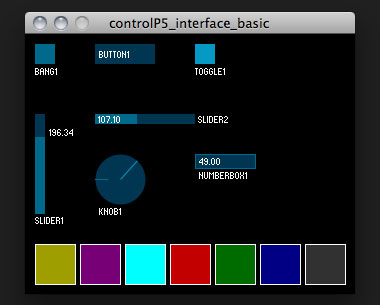
\includegraphics[width=8cm]{gambar/controlp5.jpg}
	\caption{Grafik Pengujian Koordinat X}
	\label{pic.koordinatx}
\end{figure}

Dari hasil pengujian yang ditampilkan pada Tabel \ref{tbl.koordinatx} dan juga Gambar \ref{pic.koordinatx} terlihat bahwa posisib \textit{end-effector} yang dihasilkan pada robot SCARA dibandingkan dengan data sesuai perhitungan kinematika memiliki sedikit perbedaan pada beberapa data. Perbedaan data ini dapat ditolerasi karena dengan \textit{sampling} koordinat X yang diuji hanya kurang dari lima persen nilai data yang berbeda. Pada hasil yang ditunjukkan diketahui bahwa posisi \textit{end-effector} memiliki batas minimum dan juga maksimum. Batas minimum posisi \textit{end-effector} pada sumbu X yaitu 10 cm dari titik pusat dan batas maksimum posisi \textit{end-effector} pada posisi sumbu X adalah 60 cm yang merupakan panjang dari lengan \textit{shoulder} dan juga lengan \textit{elbow}. 

\subsubsection{Pengujian Koordinat Y}
Pengujian koordinat Y dilakukan untuk mengetahui batas minimal dan batas maksimal \textit{end-effector} dari \textit{arm manipulator} robot SCARA relatif terhadap sumbu Y. Pengujian koordinat Y dilakukan dengan cara mengujicobakan setiap titik dari 0 cm sampai dengan total panjang \textit{shoulder} dan \textit{elbow} yaitu 60 cm menggunakan perhitungan kinematika balik. Perhitungan posisi Y diujicobakan menggunakan program Processing IDE, sementara untuk pengukuran posisi diukur secara faktual dari posisi \textit{end-effector} dengan membuat sebuah diagram kartesius. Tabel \ref{tbl.koordinaty} menunjukkan pengujian koordinat Y dan Gambar \ref{pic.koordinaty} menunjukkan grafik dari sampling koordinat Y.
 \begin{table}[H]
 	\centering
 	\caption{Hasil Pengujian Koordinat X}
 	\label{tbl.koordinaty}
 	\begin{tabular}{|c|l|}
 		\hline
 		\rowcolor[HTML]{9B9B9B} 
 		
 		No & \multicolumn{1}{c|}{\cellcolor[HTML]{9B9B9B}Keterangan} \\ \hline
 		1  & Robot Lengan SCARA                                      \\ \hline
 		2  & Box Panel                                               \\ \hline
 		3  & Arduino Mega 2560                                       \\ \hline
 		4  & Personal Computer                                       \\ \hline
 		5  & GUI Processing IDE                                      \\ \hline
 		6  & Workspace Robot SCARA                                   \\ \hline
 		7  & Kompresor                                               \\ \hline
 		8  & Objek                                                   \\ \hline
 	\end{tabular}
 	
 \end{table} 
 \begin{figure}[H]
 	\centering
 	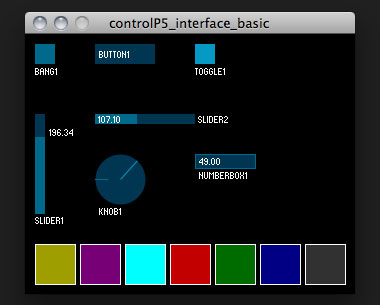
\includegraphics[width=8cm]{gambar/controlp5.jpg}
 	\caption{Grafik Pengujian Koordinat X}
 	\label{pic.koordinaty}
 \end{figure}


Dari hasil pengujian yang ditampilkan pada Tabel \ref{tbl.koordinaty} dan juga Gambar \ref{pic.koordinaty} terlihat bahwa posisi \textit{end-effector} yang dihasilkan pada robot SCARA dibandingkan dengan data sesuai perhitungan kinematika memiliki sedikit perbedaan pada beberapa data. Perbedaan data ini dapat ditolerasi karena dengan \textit{sampling} koordinat Y yang diuji hanya kurang dari lima persen nilai data yang berbeda. Pada hasil yang ditunjukkan diketahui bahwa posisi \textit{end-effector} memiliki batas minimum dan juga maksimum. Batas minimum posisi \textit{end-effector} pada sumbu Y yaitu 0 cm dari titik pusat dan batas maksimum posisi \textit{end-effector} pada posisi sumbu X adalah 60 cm yang merupakan panjang dari lengan \textit{shoulder} dan juga lengan \textit{elbow}. 

\subsubsection{Pengujian \textit{Joint Shoulder}}
Pengujian \textit{joint shoulder} dilakukan dengan membandingkan nilai sudut yang dihasilkan oleh perhitungan kinematika yang ada pada program processing IDE dengan sudut yang dihasilkan dalam aktual robot SCARA. Pengujian dilakukan dengan cara memberikan sebuah posisi koordinat X dan Y dengan nilai yang bervariasi. Nilai tersebut dimasukkan ke dalam sebuah perhitungan kinematika balik yang ada pada program Processing IDE. Hasil yang dihasilkan oleh perhitungan merupakan nilai sudut dari \textit{joint shoulder} dan juga \textit{elbow}. Perhitungan aktual dilakukan dengan cara mengukur sudut pada setiap \textit{joint} menggunakan bantuan busur atau \textit{software} sensor kemiringan yang di-\textit{install} pada smartphone. Tabel \ref{tbl.jointshoudler} merupakan hasil pengujian dari \textit{joint shoulder} berdasarkan \textit{sampling} posisi yang diambil. Gambar \ref{pic.jointshoulder} merupakan grafik hubungan dari sudut aktual dan sudut berdasarkan perhitungan kinematika. 

\begin{table}[H]
	\centering
	\caption{Hasil Pengujian \textit{Joint Shoulder}}
	\label{tbl.jointshoulder}
	\begin{tabular}{|c|l|}
		\hline
		\rowcolor[HTML]{9B9B9B} 
		
		No & \multicolumn{1}{c|}{\cellcolor[HTML]{9B9B9B}Keterangan} \\ \hline
		1  & Robot Lengan SCARA                                      \\ \hline
		2  & Box Panel                                               \\ \hline
		3  & Arduino Mega 2560                                       \\ \hline
		4  & Personal Computer                                       \\ \hline
		5  & GUI Processing IDE                                      \\ \hline
		6  & Workspace Robot SCARA                                   \\ \hline
		7  & Kompresor                                               \\ \hline
		8  & Objek                                                   \\ \hline
	\end{tabular}
	
\end{table} 
\begin{figure}[H]
	\centering
	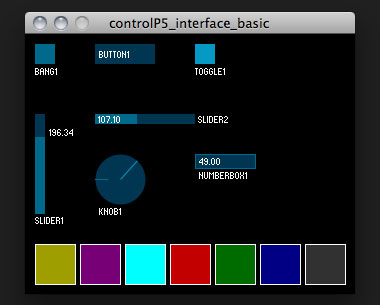
\includegraphics[width=8cm]{gambar/controlp5.jpg}
	\caption{Grafik Pengujian \textit{Joint Shoulder}}
	\label{pic.jointshoulder}
\end{figure}

Pada hasil yang ditunjukkan oleh Tabel \ref{tbl.jointshoulder} dan Gambar \ref{pic.jointshoulder} terlihat bahwa secara keseleuruhan nilai sudut yang dihasilkan oleh aktual pada robot SCARA dibandingkan dengan perhitungan kinematika oleh Processing IDE tidak begitu terdapat perbedaan. Terlihat bahwa nilai error
 memiliki nilai minimum .... persen dan nilai maksimum ... persen. Persentase error didapat dari data yang tidak sesuai dibagi oleh keleluruhan data yang diuji coba. 
 
 \subsubsection{Pengujian \textit{Joint Elbow}}
 Pengujian \textit{joint elbow} dilakukan dengan membandingkan nilai sudut yang dihasilkan oleh perhitungan kinematika yang ada pada program processing IDE dengan sudut yang dihasilkan dalam aktual robot SCARA. Pengujian dilakukan dengan cara memberikan sebuah posisi koordinat X dan Y dengan nilai yang bervariasi. Nilai tersebut dimasukkan ke dalam sebuah perhitungan kinematika balik yang ada pada program Processing IDE. Hasil yang dihasilkan oleh perhitungan merupakan nilai sudut dari \textit{joint shoulder} dan juga \textit{elbow}. Perhitungan aktual dilakukan dengan cara mengukur sudut pada setiap \textit{joint} menggunakan bantuan busur atau \textit{software} sensor kemiringan yang di-\textit{install} pada smartphone. Tabel \ref{tbl.jointelbow} merupakan hasil pengujian dari \textit{joint elbow} berdasarkan \textit{sampling} posisi yang diambil. Gambar \ref{pic.jointelbow} merupakan grafik hubungan dari sudut aktual dan sudut berdasarkan perhitungan kinematika. 
 
 \begin{table}[H]
 	\centering
 	\caption{Hasil Pengujian \textit{Joint Elbow}}
 	\label{tbl.jointelbow}
 	\begin{tabular}{|c|l|}
 		\hline
 		\rowcolor[HTML]{9B9B9B} 
 		
 		No & \multicolumn{1}{c|}{\cellcolor[HTML]{9B9B9B}Keterangan} \\ \hline
 		1  & Robot Lengan SCARA                                      \\ \hline
 		2  & Box Panel                                               \\ \hline
 		3  & Arduino Mega 2560                                       \\ \hline
 		4  & Personal Computer                                       \\ \hline
 		5  & GUI Processing IDE                                      \\ \hline
 		6  & Workspace Robot SCARA                                   \\ \hline
 		7  & Kompresor                                               \\ \hline
 		8  & Objek                                                   \\ \hline
 	\end{tabular}
 	
 \end{table} 
 \begin{figure}[H]
 	\centering
 	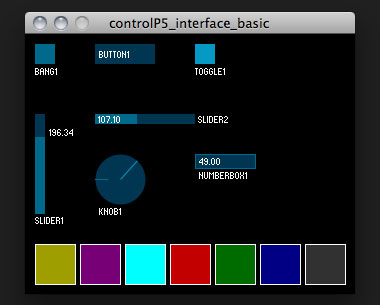
\includegraphics[width=8cm]{gambar/controlp5.jpg}
 	\caption{Grafik Pengujian \textit{Joint Elbow}}
 	\label{pic.jointelbow}
 \end{figure}
 
 Pada hasil yang ditunjukkan oleh Tabel \ref{tbl.jointelbow} dan Gambar \ref{pic.jointelbow} terlihat bahwa secara keseleuruhan nilai sudut yang dihasilkan oleh aktual pada robot SCARA dibandingkan dengan perhitungan kinematika oleh Processing IDE tidak begitu terdapat perbedaan. Terlihat bahwa nilai error
 memiliki nilai minimum .... persen dan nilai maksimum ... persen. Persentase error didapat dari data yang tidak sesuai dibagi oleh keleluruhan data yang diuji coba. 